\renewcommand{\baselinestretch}{1.25}%
\begin{figure}[!t]%
  \centering
  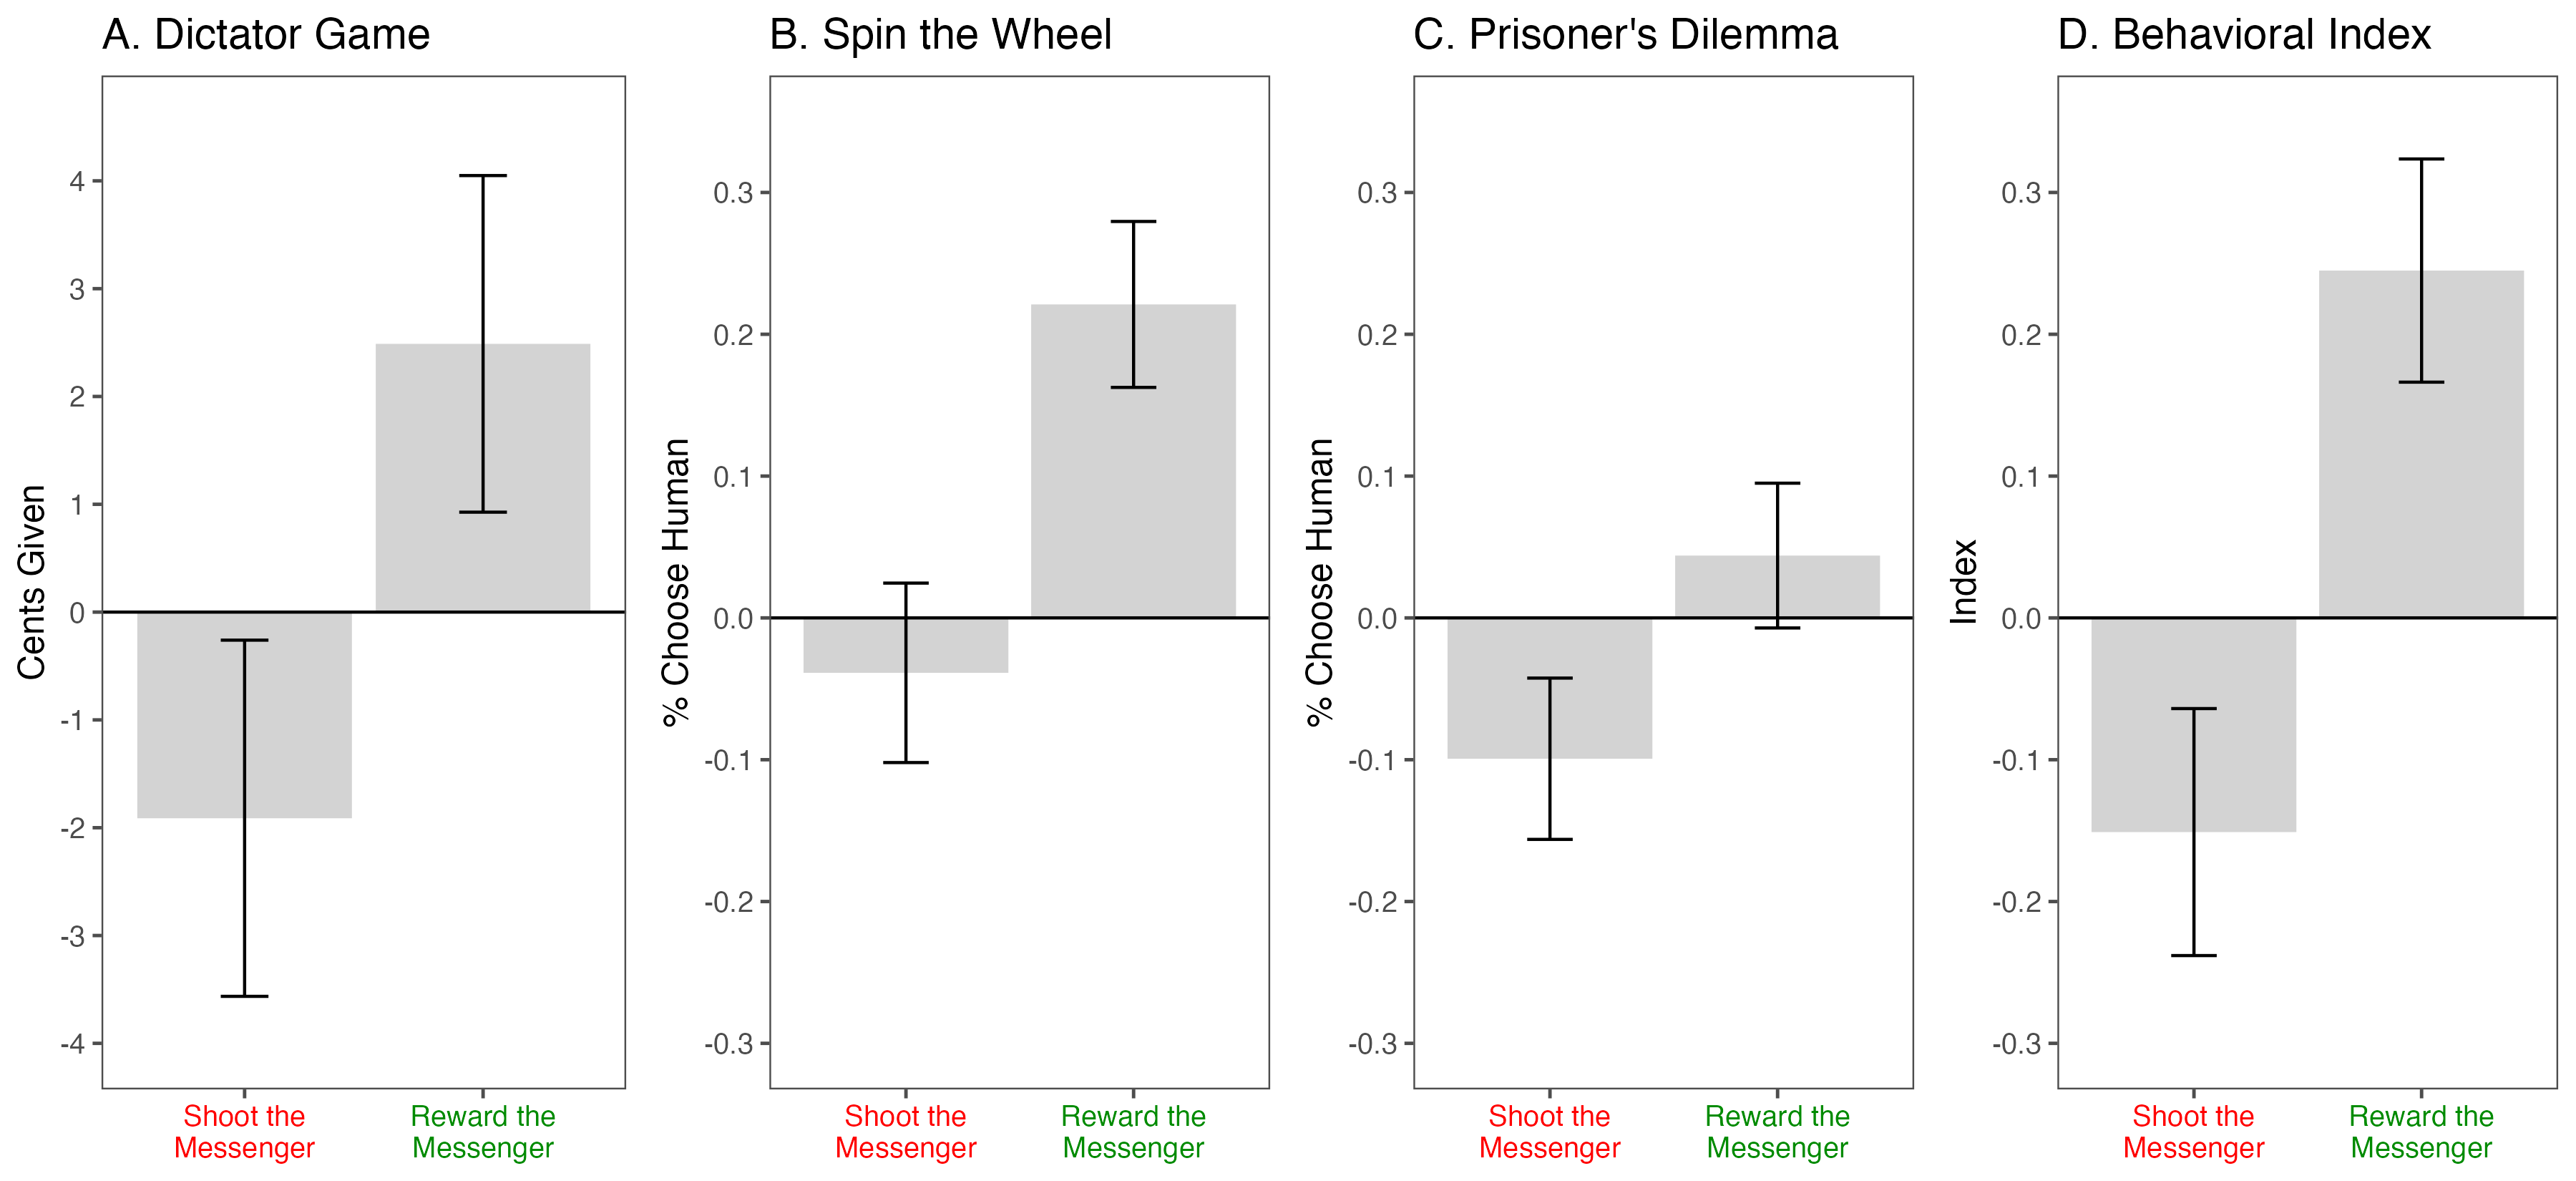
\includegraphics[width=1.0\textwidth]{figures/study1_behavior_list.png}
  \caption{Difference in the DVs of the behavior measures for messengers and non-messengers 
                                              by losing (STM) and winning (RTM), Study 1. 
  \textit{Note: OLS regression with robust standard errors, with error bars representing 95\% confidence intervals. In the dictator game (Panel A), the dependent variable (DV) is giving up to 50 cents to the partner. 
                 In the spin the wheel task (Panel B), the DV is choosing the partner to spin the wheel on one’s behalf instead of the computer. 
                 In the prisoner’s dilemma (Panel C), the DV is choosing cooperation. 
                 In the behavioral index (Panel D), the DV is calculated by averaging the standardized scores of the dictator game, spin the wheel task, and prisoner's dilemma. The p-values of the test that $RTM = -STM$ are 0.62, 0.00, 0.16, and 0.12, respectively, for each facet and the index. The p-values of the messenger bias are 0.00, 0.00, 0.00, and 0.00, respectively, for each facet and the index.}}
  \label{fig:behavior_list}
\end{figure}%
\renewcommand{\baselinestretch}{1.67}%
